\documentclass[brazil]{beamer}
\usepackage[utf8]{inputenc}
\usepackage[T1]{fontenc}
\usepackage{lmodern}
\usepackage{graphicx}			%para imagens
\usepackage{epstopdf} 			%resolve problemas eps-pdf
\usepackage{fancyhdr}			% para o cabeçalho bonito
\usepackage{caption}				%para legendas
\usepackage{placeins} 			%controlar o lugar dos floats
\usepackage{color}
\usepackage{url}
\usepackage{bm}
\renewcommand{\UrlFont}{\tiny}
\usepackage{relsize}
\usepackage{hyperref}

\usetheme{Dresden}
\usecolortheme{orchid}
\setbeamertemplate{navigation symbols}{}

\newcommand{\HRule}{\rule{\linewidth}{0.5mm}}

\title{EZ3D: Rastreamento Visual de Movimentos Faciais sem Marcadores para Modelos de Animação Tridimensionais}
\author{Juarez Aires Sampaio Filho \\ Rodrigo de Assis Ramos Lima}
\titlegraphic{\leavevmode\smash{\raisebox{5.5cm}{
\includegraphics[width=0.8\textwidth]{./img/logo.jpg}}}}
\institute{Universidade de Brasília}
\date{8 de Dezembro de 2016}


\begin{document}
\begin{frame}
        \titlepage
\end{frame}

\begin{frame}[fragile]
  \frametitle{Conteúdo}
  \begin{itemize}
     \item Introdução
     \begin{itemize}
     	\item O Mercado de Animação
     	\item Técnicas para Transferência de Movimentos
    	 	\item Motivação
   	 \end{itemize}
     \item Metodologia Utilizada
     \begin{itemize}
    	 	\item Rastreamento de Pontos do Rosto
    	 	\item Estimação de Tridimensionalidade e Filtros Digitais
    	 	\item Mistura de Poses
   	 \end{itemize}
     \item Resultados
     \begin{itemize}
    	 	\item Rastreamento de Pontos do Rosto
    	 	\item Estimação de Tridimensionalidade e Filtros Digitais
    	 	\item Resultado Final
   	 \end{itemize}
     \item Conclusões
  \end{itemize}
\end{frame}

\begin{frame}[fragile]
  \frametitle{Introdução}

  \begin{itemize}
      \item O Mercado de Animação:
      
      \begin{itemize}
      
        \item O mercado global de animação e jogos foi avaliado em \$122.20 bilhões em 2010 e é esperado que esta cifra atinja  \$242.93 bilhões em 2016.
        
        \item Este mercado pode ser subdividido em várias categorias sendo \textbf{Filmes} e \textbf{Efeitos Visuais} categorias de especial interesse para este trabalho.
        
        \item As técnicas de animação tridimensional ainda apresentam custos elevados e proibitivos para certas aplicações. Ela é em si uma técnica \textbf{cara}.
          
  \end{itemize} 
      
          
  \end{itemize}

\end{frame}
\begin{frame}
      \begin{figure}
        \centering
        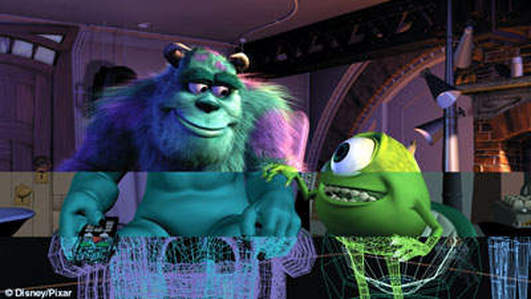
\includegraphics[width = 0.9\textwidth, keepaspectratio]{./img/sully.jpg}
        \caption{Foram utilizados mais de 2 milhões de fios de cabelo individualmente nomeados para a construção do personagem \textit{Sully}. Um único quadro com o personagem custou em média de 11 a 12 horas de trabalho criativo.}
      \end{figure}
\end{frame}

\begin{frame}

\begin{itemize}
      \item Técnicas para Transferência de Movimentos:
      
      \begin{itemize}
      
        \item Uma técnica importante que vem ao auxílio dos animadores consiste em transferir movimentos e expressões de um ator para um modelo computacional.
        
        \item Metodologias para captura ótica de \textbf{performance teatral} são utilizadas na indústria já há algum tempo.
        
        \item Outro recurso utilizado para a animação auxiliada por captura de vídeo é o uso de fantoches digitais, mas neste caso os requisitos de \textbf{tempo} são muito mais severos.
        
      \end{itemize}   
          
  \end{itemize} 
	
\end{frame}

\begin{frame}
  \frametitle{Imagem do Smaug}

\end{frame}

\begin{frame}
  \begin{itemize}
      \item Motivação:
      
      \begin{itemize}
      
        \item Apesar das soluções existentes apresentarem resultados adequados para as aplicações citadas, elas apresentam um \textbf{alto custo}. Esse custo se torna proibitivo para aplicações desenvolvidas por pequenas empresas.
        
        \item Um produto de baixo custo poderia, por exemplo, ser utilizado por \textbf{animadores independentes} para acelerar seus projetos.
        
        \item Programas de televisão educacionais para crianças abundam no mercado, mas são em sua maioria direcionados ao público infantil geral. Um nicho não atendido é o de
\textbf{crianças autistas}.
        
      \end{itemize}   
          
  \end{itemize} 

\end{frame}

\begin{frame}
  \begin{itemize}
      \item Motivação:
      
      \begin{itemize}
      
        \item Apesar das soluções existentes apresentarem resultados adequados para as aplicações citadas, elas apresentam um \textbf{alto custo}. Esse custo se torna proibitivo para aplicações desenvolvidas por pequenas empresas.
        
        \item Um produto de baixo custo poderia, por exemplo, ser utilizado por \textbf{animadores independentes} para acelerar seus projetos.
        
        \item Programas de televisão educacionais para crianças abundam no mercado, mas são em sua maioria direcionados ao público infantil geral. Um nicho não atendido é o de
\textbf{crianças autistas}.
        
      \end{itemize}   
          
  \end{itemize} 

\end{frame}



\end{document}
